\section{Решение}

Данная фигура строится в два этапа: Для начала берется некий круг в основании, где в цикле многогранником приближенно отображается основание пирамиды. Далее, для каждой стороны этого многогранника строится треугольник, который соеденяет основание с вершиной пирамиды, которая задается расстоянием от основания, также как и радиус основания, он передается в функцию отображения.


% % \usepackage[rightcaption]{sidecap}

% \usepackage{graphicx} %package to manage images
% % \graphicspath{ {images/} 

% \begin{SCfigure}[0.5][h]
% \caption{Using again the picture of the universe.
% This caption will be on the right}
% 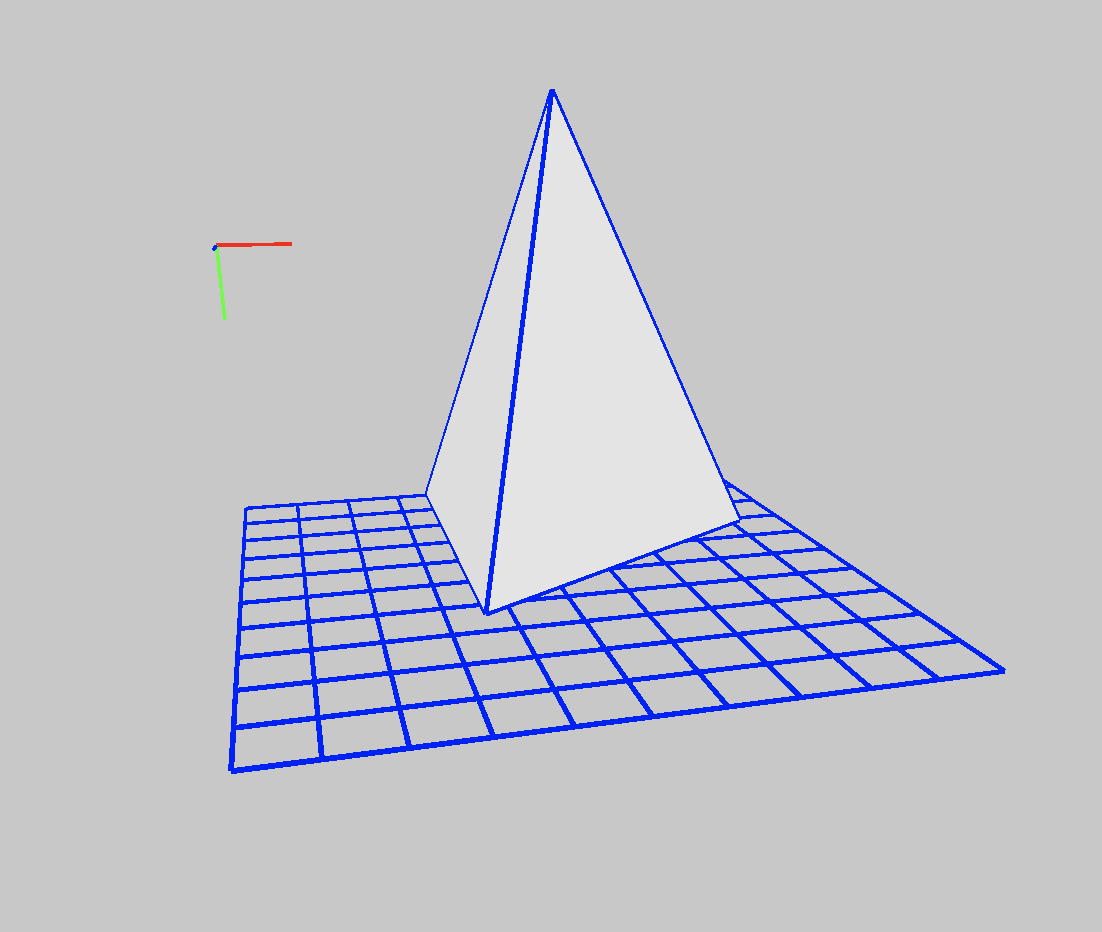
\includegraphics[width=0.6\textwidth]{pictures/2.png}
% \end{SCfigure}

Ползунком n регулируется количество сторон (от 3 до 6).


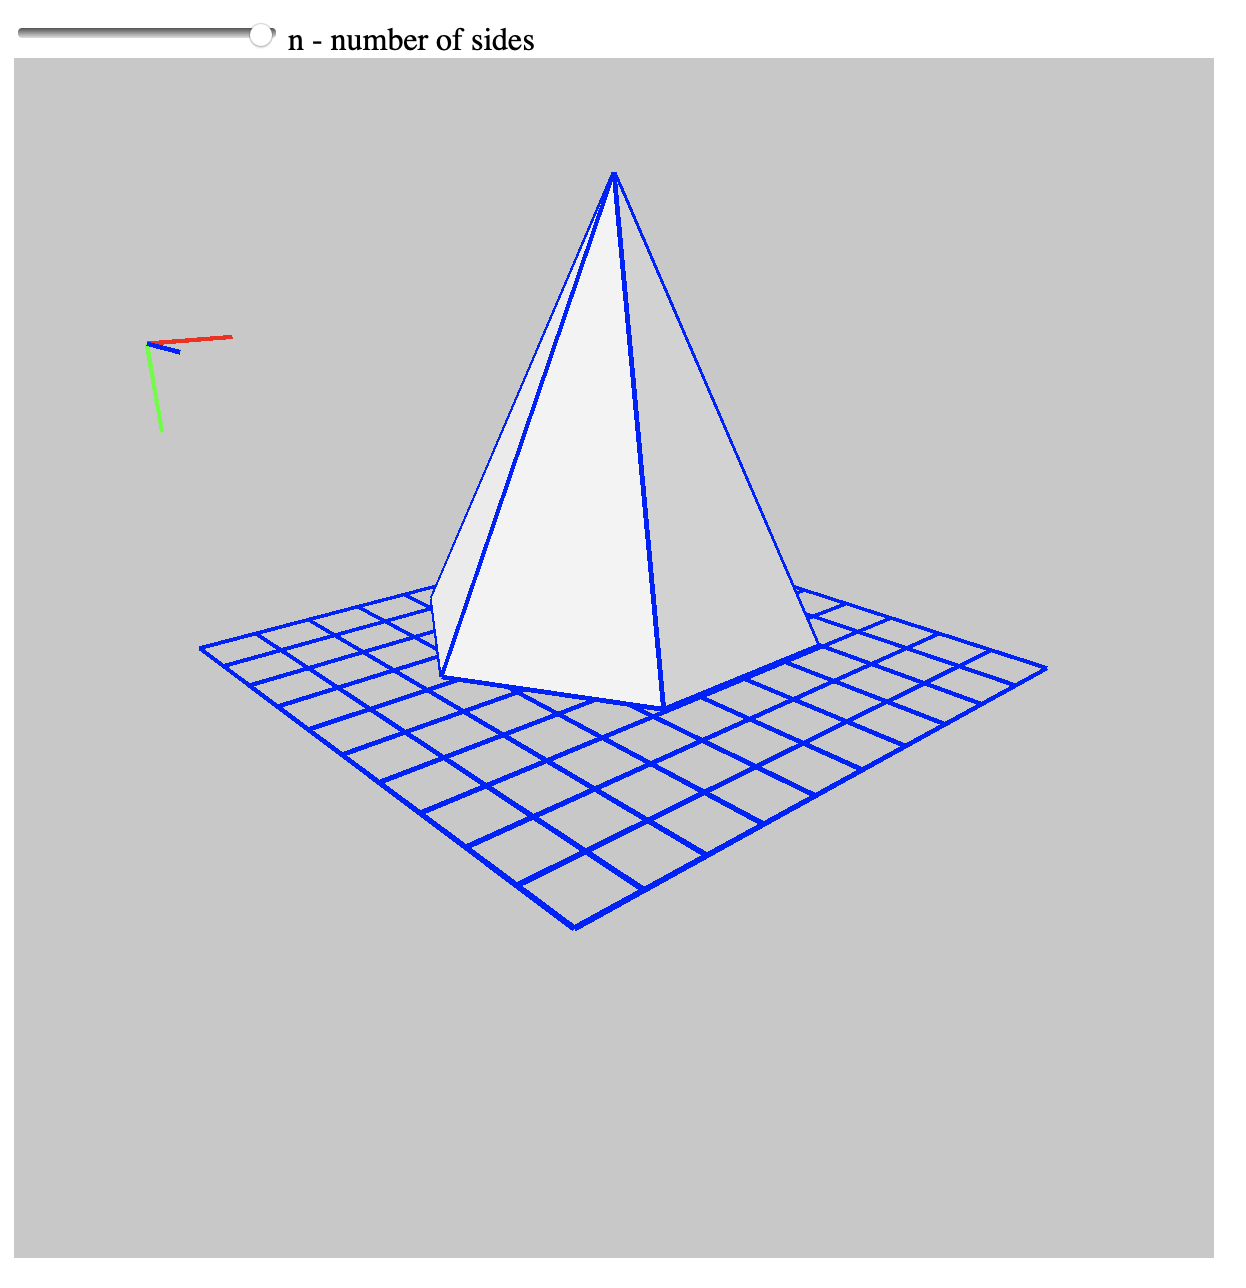
\includegraphics[scale=0.5]{pictures/3.png}

Приведена пирамида для 6 боковых сторон.

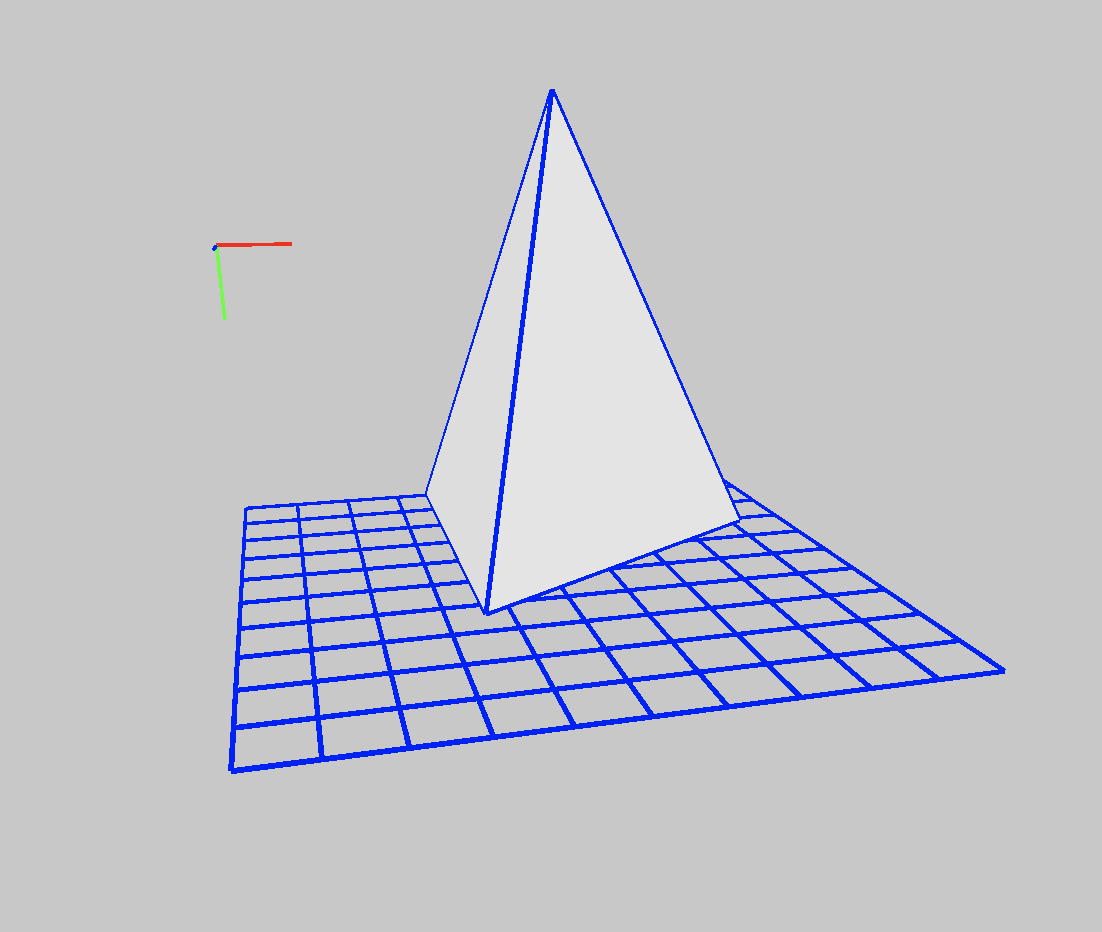
\includegraphics[scale=0.4]{pictures/2.png}

Приведена пирамида для 3 боковых сторон.

% \section{Исходный код}

% \begin{lstlisting}[language=C++]
% \end{lstlisting}

% \lstset{language=[gnu] make}
% \lstset{
%   language=[gnu] make,
%   keywordstyle=\color{teal}\textbf,
%   stringstyle=\color{blue},
%   identifierstyle=\itshape
% }

% \begin{lstlisting}
% CC = g++
% CCFLAGS = -std=c++14 -Wall -pedantic -O3
% ###____###
% solution : main.cpp *.hpp ; $(CC) $(CCFLAGS) main.cpp -o solution
% clean	 : ;
% \end{lstlisting}

% \section{Консоль}

% \begin{alltt}
% \end{alltt}

% \pagebreak